\documentclass[a4paper,12pt,obeyspaces,spaces,hyphens]{article}

\def \trainingtype{online}
\def \agendalanguage{french}

\input{agenda/yocto.inc}

\usepackage{agenda}

\begin{document}

\feshowtitle

\feshowinfo

\feagendatwocolumn
{Plateforme matérielle pour les démonstrations, option \#1}
{
  Une de ces cartes de STMicroelectronics : {\bf
  STM32MP157A-DK1}, {\bf STM32MP157D-DK1}, {\bf STM32MP157C-DK2} ou
  {\bf STM32MP157F-DK2}
  \begin{itemize}
  \item Processeur STM32MP157, double Cortex-A7, de STMicroelectronics
  \item Alimentée par USB
  \item 512 Mo DDR3L RAM
  \item Port Gigabit Ethernet port
  \item 4 ports hôte USB 2.0
  \item 1 port USB-C OTG
  \item 1 connecteur Micro SD
  \item Debugger ST-LINK/V2-1 sur la carte
  \item Connecteurs compatibles Arduino Uno v3
  \item Codec audio
  \item Divers : boutons, LEDs
  \item Écran LCD tactile (uniquement sur cartes DK2)
  \end{itemize}
}
{}
{
  \begin{center}
    \includegraphics[width=5cm]{../slides/discovery-board-dk1/discovery-board-dk1.png}
  \end{center}
}

\feagendatwocolumn
{Plateforme matérielle pour les démonstrations, option \#2}
{
  Carte {\bf BeagleBone Black} ou {\bf BeagleBone Black Wireless}
  \begin{itemize}
  \item Un processeur ARM AM335x de Texas Instruments (à base de
    Cortex-A8), avec accélération 3D, etc.
  \item 512 Mo de RAM
  \item 2 ou 4 Go de stockage eMMC
  \item USB hôte et device
  \item Sortie HDMI
  \item Connecteurs à 2 x 46 broches, pour accéder aux UARTs, aux bus
    SPI, aux bus I2C, et à d'autres entrées/sorties du processeur.
  \item Ethernet ou WiFi
  \end{itemize}
}
{}
{
  \begin{center}
    \includegraphics[width=5cm]{../slides/beagleboneblack-board/beagleboneblack.png}
  \end{center}
}

\feagendatwocolumn
{Plateforme matérielle pour les travaux pratiques, option \#3}
{
  Carte {\bf BeaglePlay}
  \begin{itemize}
    \item SoC Texas Instruments AM625x (CPU 4xARM Cortex-A53)
    \item SoC avec accélération 3D, MCU intégré et de nombreux autres périphériques.
    \item 2 GB de RAM
    \item 16 Go de stockage eMMC
    \item USB hôte et device, microSD, HDMI
    \item WiFi 2.4 and 5 GHz, Bluetooth et aussi Ethernet
    \item 1 Header MicroBus (SPI, I2C, UART, ...), connecteurs OLDI et CSI.
  \end{itemize}
}
{}
{
  \begin{center}
    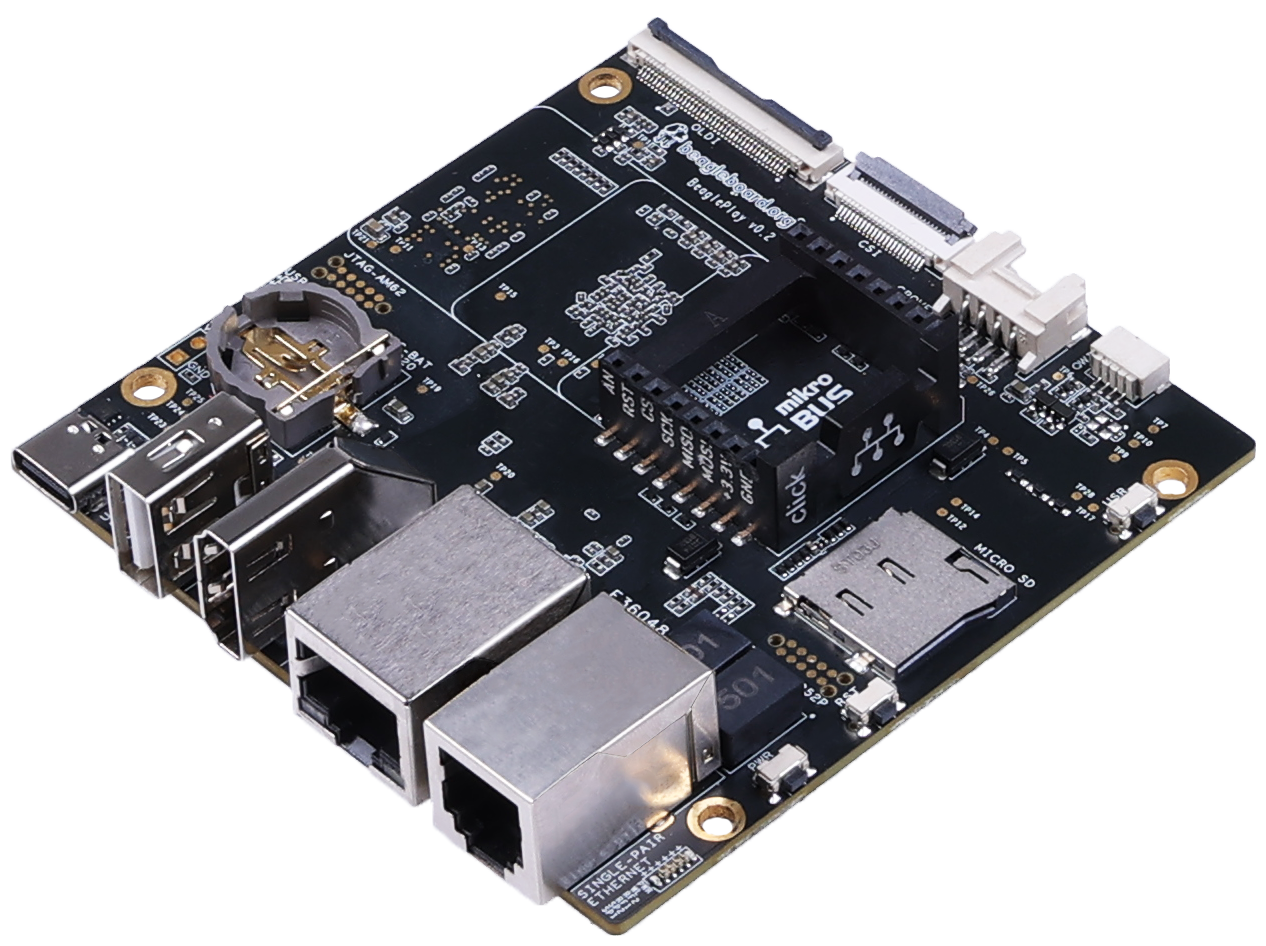
\includegraphics[width=5cm]{../slides/beagleplay-board/beagleplay.png}
  \end{center}
}

\section{1\textsuperscript{ère} demi-journée}

\feagendaonecolumn
{Cours - Introduction aux outils de compilation de systèmes Linux embarqué}
{
  \begin{itemize}
  \item Vue d'ensemble de l'architecture d'un système Linux embarqué
  \item Méthodes pour compiler un système de fichiers
  \item Utilité des outils de compilation
  \end{itemize}
}

\feagendaonecolumn
{Cours - Vue d'ensemble de Yocto Project et du système de référence Poky}
{
  \begin{itemize}
  \item Présentation de l'outil de compilation Yocto / OpenEmbedded et de sa terminologie.
  \item Vue d'ensemble du système de référence Poky
  \end{itemize}
}

\feagendatwocolumn
{Cours - Bases de l'utilisation de Yocto Project}
{
  \begin{itemize}
  \item Mise en place du répertoire de travail et de l'environnement
  \item Configuration de l'outil de compilation
  \item Compilation de l'image d'un système de fichiers racine
  \end{itemize}
}
{Démo 1 - 1\textsuperscript{ère} compilation avec Yocto Project}
{
  \begin{itemize}
  \item Téléchargement du système de référence Poky
  \item Configuration de l'outil de compilation
  \item Compilation d'une image système
 \end{itemize}
}

\feagendatwocolumn
{Cours - Utilisation de Yocto Project - Notions de base}
{
  \begin{itemize}
  \item Structure des fichiers générés
  \end{itemize}
}
{Démo 1 - Flasher et booter}
{
  \begin{itemize}
  \item Flasher et booter l'image du système sur la carte
  \end{itemize}
}

\section{2\textsuperscript{ème} demi-journée}

\feagendatwocolumn
{Cours - Utilisation de Yocto Project - Utilisation avancée}
{
  \begin{itemize}
  \item Assignation des variables, opérateurs et surcharge
  \item Paquetages: variantes de paquetages
  \item Options de la commande bitbake
  \end{itemize}
}
{Démo 2 - Utilisation de NFS et configuration de la compilation}
{
  \begin{itemize}
  \item Configurer la carte pour démarrer via NFS
  \item Rajouter un paquetage au système de fichiers racine
  \item Apprendre à utiliser le mécanisme \code{PREFERRED_PROVIDER}
  \item Se familiariser avec les options de la commande bitbake
  \end{itemize}
}
\\

\feagendatwocolumn
{Cours - Écriture de recettes - Fonctionnalités de base}
{
  \begin{itemize}
  \item Recettes: vue d'ensemble
  \item Organisation d'un fichier de recette
  \item Application de patches
  \item Exemples de recettes
  \end{itemize}
}
{Démo 3 - Ajouter la compilation d'une application}
{
  \begin{itemize}
  \item Création d'une recette pour {\em nInvaders}
  \item Résolution de problèmes liés à la recette
  \item Résolution de problèmes liés à la compilation croisée
  \item Ajout d'{\em nInvaders} à l'image finale
  \end{itemize}
}

\feagendaonecolumn
{Cours - Écriture de recettes - Fonctionnalités avancées}
{
  \begin{itemize}
  \item Extension et redéfinition de recettes
  \item Paquetages virtuels
  \item Familiarisation avec les classes
  \item Inclusion d'exemples avec BitBake
  \item Mise au point des recettes
  \item Configuration de l'utilisation du réseau par BitBake
  \end{itemize}
}

\section{3\textsuperscript{ème} demi-journée}

\feagendatwocolumn
{Cours - Layers}
{
  \begin{itemize}
  \item Ce que sont les {\em layers}
  \item Où trouver les {\em layers}
  \item Création d'un {\em layer}
  \end{itemize}
}
{Démo 4 - Écriture d'un layer}
{
  \begin{itemize}
  \item Apprendre à écrire un {\em layer}
  \item Ajouter le {\em layer} à la compilation
  \item Inclure {\em nInvaders} dans le nouveau {\em layer}
  \end{itemize}
}

\feagendaonecolumn
{TP 5 - Étendre une recette}
{
  \begin{itemize}
  \item Étendre la recette pour le noyau pour rajouter des patches
  \item Configurer le noyau pour compiler le pilote du nunchuk
  \item Modifier la recette ninvaders pour rajouter des patches
  \item Jouer avec {\em nInvaders}
  \end{itemize}
}

\feagendatwocolumn
{Cours - Écriture d'un BSP}
{
  \begin{itemize}
  \item Introduction aux layers BSP
  \item Ajout d'une nouvelle machine
  \item Configuration du chargeur de démarrage
  \item Linux : la classe kernel.bbclass et la recette linux-yocto
  \end{itemize}
}
{Démo 6 - Création d'une configuration spécifique pour une machine}
{
  \begin{itemize}
  \item Créer un nouvelle configuration de machine
  \item Compiler une image pour la machine
  \end{itemize}
}

\feagendaonecolumn
{Cours - Layers de distribution}
{
  \begin{itemize}
  \item Configuration d'une distribution
  \item Layers de distribution
  \end{itemize}
}

\feagendatwocolumn
{Cours - Images}
{
  \begin{itemize}
  \item Écriture d'une recette d'image
  \item Types d'images
  \item Écriture et utilisation de groupes de paquetages
  \end{itemize}
}
{Démo 7 - Création d'une image sur mesure}
{
  \begin{itemize}
  \item Rajouter une recette de base pour une image
  \item Sélectionner les fonctionnalités et les paquetages de l'image
  \item Ajouter un groupe de paquetages sur mesure
  \item Ajouter une variante d'image pour le débogage
  \end{itemize}
}

\section{4\textsuperscript{ème} demi-journée}

\feagendatwocolumn
{Cours - Écriture de recettes - Pour aller plus loin}
{
  \begin{itemize}
  \item Le sysroot de chaque recette
  \item Utilisation de code Python code dans les méta-données
  \item Drapeaux de variables
  \item Fonctionnalités de paquetages et PACKAGECONFIG
  \item Fonctionnalités conditionnelles
  \item Découpage de paquetages
  \item Détails sur les dépendances
  \end{itemize}
}
{Cours - Licences}
{
  \begin{itemize}
  \item Gestion de licences open source
  \end{itemize}
}

\feagendatwocolumn
{Cours - SDK pour le projet Yocto}
{
  \begin{itemize}
  \item Objectifs du SDK
  \item Compilation et personnalisation d'un SDK
  \item Utilisation d'un SDK pour le projet Yocto
  \end{itemize}
}
{Démo 8 - Développement d'une application au moyen du SDK de Poky}
{
  \begin{itemize}
  \item Compilation d'un SDK
  \item Utilisation du SDK
  \end{itemize}
}

\feagendatwocolumn
{Cours - Devtool}
{
  \begin{itemize}
  \item Présentation devtool
  \item Cas d'utilisation de devtool
  \end{itemize}
}
{Démo 9 - Utilisation de devtool}
{
  \begin{itemize}
  \item Création d'une nouvelle recette
  \item Modification d'une recette pour ajouter un nouveau patch
  \item Mettre à jour une recette pour prendre en charge une nouvelle version
  \end{itemize}
}

\feagendatwocolumn
{Cours - Gestion automatique de layers}
{
  \begin{itemize}
  \item Gestion automatique de layers
  \end{itemize}
}
{Cours - Gestion de paquetages à l'exécution}
{
  \begin{itemize}
  \item Introduction à la gestion de paquetages à l'exécution
  \item Configuration de la compilation
  \item Configuration d'une serveur de paquetages
  \item Configuration de la machine cible
  \end{itemize}
}

\feagendaonecolumn
{Questions / réponses}
{
  \begin{itemize}
  \item Questions et réponses avec les participants à propos des sujets abordés.
  \item Présentations supplémentaires s'il reste du temps, en fonction des demandes
        de la majorité des participants.
  \end{itemize}
}

\section{Temps supplémentaire possible}

{\em Du temps supplémentaire (jusqu'à 4 heures) pourrait être proposé si le programme ne tenait
     pas en 4 demi-journées, selon le temps passé à répondre aux questions des participants.}

\end{document}
